%#!platex tls.tex
\chapter{画像と描画}

\begin{abstract}
\begin{flushright}
画像でも\\
\TeX にかかれば\\
\kenten{ただ}の箱
\end{flushright}
\end{abstract}

\section{\BB}

いかなる画像ファイルも \TeX にかかれば\kenten{ただ}の箱として扱われます.
\dvipdfmx 等で,ある型式のビットマップ画像を読み込むためには\BB ファイル
なるファイルを生成する必要があります.これは大抵 \Prog{ebb} という付属の
プログラムで作成する事が出来ます\footnote{別ファイルに用意する必要性があ
る訳ではありません.}.

\BB ファイルには最低限,ビットマップ画像の $(x_0, y_0)$ 座標と $(x, y)$
座標の組が記述されています.

\begin{InText}
%%Title: ./file.bmp
%%Creator: ebb Version 0.5.2
%%BoundingBox: 0 0 595 841
%%CreationDate: Fri Oct 03 10:03:07 2003
\end{InText}

ebb の場合はその他にファイル名 (Title),作成プログラム (Creator),
作成日時 (CreationDate) の項目があります.

同じディレクトリにある画像ファイルの \BB ファイルを生成したい時
は,次のようにすれば,PNG, PDF, JPEG の \suf{bb} がそれぞれ作成される事
でしょう.

\begin{InTerm}
  \type{ebb *.png *.pdf *.jpg}
\end{InTerm}

\TeX は画像も一つの箱としてしか見ていないので,画像の縦 $\times$ 横と原
点が分かればそれで組版できます.EPS 画像には `\str{0 0 200 300}' のような
\BB  情報が含まれているので,これを使って $200 \times 300$ の箱を
配置しています.

\begin{Prob}
実際に何かしらのプログラムで作成した EPS 画像の \BB に関する
記述を探してみてください.

\begin{InText}
%!PS-Adobe-3.0 EPSF-3.0
%%Creator: (ImageMagick)
%%Title: (gnu-head.eps)
%%CreationDate: (Thu Oct 14 23:24:09 2004)
%%BoundingBox: 0 0 276 261
%%HiResBoundingBox: 0 0 276 261
%%DocumentData: Clean7Bit
%%LanguageLevel: 1
%%Pages: 1
%%EndComments 
\end{InText}

プログラムによっては \str{BoundingBox} 以外にも \str{HiResBoundingBox}
という項目が作成されている場合があると思います.これは小数点以下も
扱う,高精度版の \BB 情報になります.
\end{Prob}

どのような画像形式であろうが,\BB  を指定さえすれば, \TeX は正確
に組版できます.
%\begin{InText}
% \includegraphics[bb= 0 0 200 300]{hoge.xxx}
%\end{InText}
%
そして,実際に画像を取り扱うのは 「デバイスドライバ」であって,このデバ
イスドライバの能力に依存して取り込める画像形式が決まります.

%dvipsk などであれば EPS などであろう. \dviout は Susie plugin と組み合
%わせれば,ほとんどの画像形式を読み込む事が出来る.PDF を生成する
%\dvipdfmx であれば,BMP, JPEG, PNG, PDF, EPS, MetaPost などが読み込める.

\subsection{正確な\BB の測定}

時折,\GS などが正確な \BB  が実際の描画領域を取得してく
れない事があるので,PSTricks を使用している時に問題になる事があります.
PSTricks で例えば何らかの図形を描いて,それを dvips で
\begin{InTerm}
  \type{dvips -Ppdf -o fig1.eps input.dvi}
\end{InTerm}
とすると \fl{fig1.eps} が作成されます.こいつの真の \BB  を取得す
るには
\begin{InTerm}
  \type{gs -sDEVICE=pbm fig1.eps -sOutputFile=fig1.pbm}
  \type{bbb < fig1.pbm > fig1.bb}
\end{InTerm}
などとすると良いでしょう.
\Prog{bbb} は \BB  を割り出すようなプログラム,例えば次のようなも
のです.

\lstinputlisting[language=Perl]{bbb}

通常は EPS に記述されているヘッダーの\BB 情報だけを取得するので
\begin{InText}
%%BoudingBox: 0 0 300 200 
\end{InText}
というコメント行があれば,それしか参照しません.しかし,
\begin{InText}
 draw circle (300, 200, 10);
\end{InText}
のように $(300, 200)$ の座標に直径10\,pt の円を描け,という場合には対応
できません.ですから,正確な \BB  を取得するためには実際にその画像が最終
的にどのように描かれるのかを知らなければならないということになります.

通常の \BB  を算出するようなプログラムは線のギリギリの部分で\BB  を取ろ
うとするので,線が欠けてしまう事があります.

上記で提案しているプログラムは線が欠けてしまわないように,それぞれ
上下左右に1\,ptのマージンを加えてあります.

\section{描画の方法}

コンピュータにおける描画の方法の基本的な事項は初級編の
第6章で既に解説しておりますので,まだご覧になっておられないのであれば,
そちらを参照してください.初級編では\Y{graphicx}パッケージを用いて,
既に作成された画像アイルをどのように張り込むかの手順を説明しています.

周辺ツール編では\E{picture}環境等の\LaTeX での描画ではなく,他のプログラ
ムの活用方法に焦点を当てます.ただし,そのプログラムの基本的な使い方の説
明ではなく,どのようにすれば \LaTeX とうまく連携できるのかを中心に説明し
ます.



\section{Windows用の描画ソフト}

\subsection{WinTpic}

\Hito{堀井}{雅司}により作成された\Prog{WinTpic}は,
\TeX と非常に親和性の高いプログラムです.GUI で \Tpic の描画を行なう事
が出来ると思って良いと思います\footnote{\Tpic については初級編の第6章を
参照してください.}.

\image[scale=.4]{wintpic}{WinTpicの起動例}{wintpic}

% HOGE r か l かどっちだよ.自動的にやろうかなぁ.
\begin{wrapfigure}[10]{l}{16zw}
 \centering
 \input{images/wintpic-smpl.wtp}
 \caption{WinTpicの描画例}\figlab{wintpic-smpl}
\end{wrapfigure}

線や楕円,多角形等の図形要素描画,\TeX 文字列の挿入,指数関数,
対数関数,三角関数等の各種関数の描画,領域の塗りつぶしなどの
機能があります.

適切に図を作成したならば,原稿中で \C{input} 命令で然るべき場所にて
保存したファイル \fl{input-sample.tex} を読み込むだけです.

WinTpic では図形を\E{picture}環境の中に入れています.
このため,文字列等は \C{put}命令と \C{makebox}命令により
配置する場所を決めています.

WinTpic 上で配置した文字列を実際に \LaTeX でタイプセットすると若干
ずれる事がありますので,微調整が必要になる場合があるかと思います.
WinTpic 側に \LaTeX プレビューの機能がありますので,dviout をプレビュー
アとして確認作業を行なうが良いと思われます.


\subsection{EPS-draw}

EPS-draw は \Hito{寺嶋}{容明}によって作成された描画プログラムです.

\begin{wrapfigure}{r}{27zw}
 \centering
 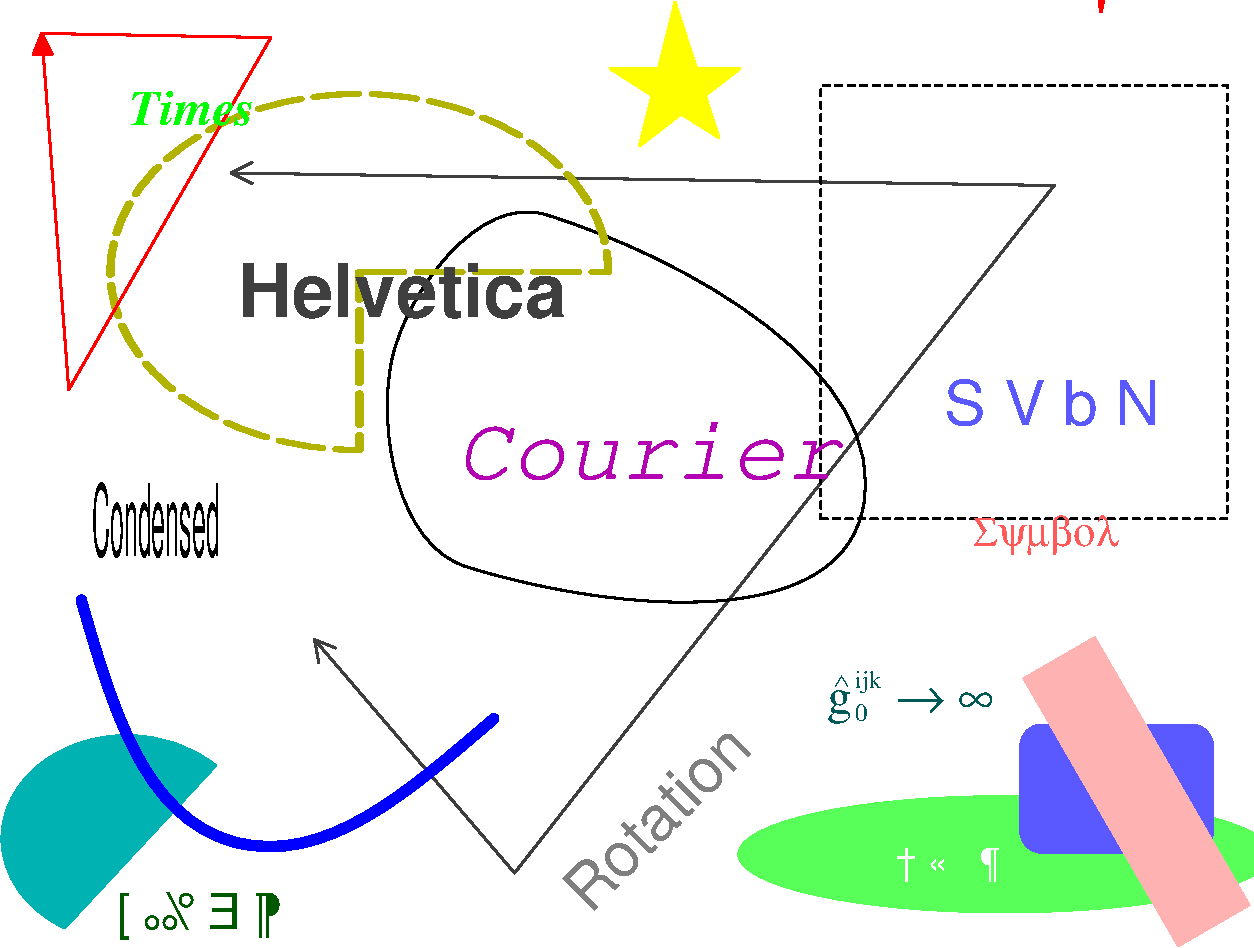
\includegraphics[scale=.4]{images/EPSdraw-crop}
 \caption{EPS-drawの描画例}\figlab{eps-draw}
\end{wrapfigure}

描画内容を直接 EPS に出力する事が出来ます.\hito{寺嶋}{容明}は
\Prog{EPS-draw} 以外にも \Prog{EPS-conv}, \Prog{EPS-merg},
\Prog{PushGsRg}等のプログラムを作成しています.

EPS-drawでは直線,曲線,楕円,多角形等の図形要素の配置,文字の配置,色の
指定などが出来る優れた描画プログラムです.

フォントもHelvetica, Times, Symbol, Courier等を扱う事が出来ます.日本語に
おいては明朝体とゴシック体の両方を扱えます.

EPS-draw は \suf{edf}というファイル形式でファイルを保存します.
「EPS出力」を選択する事でEPS画像をエキスポートできます.



\subsection{Dynamic Draw}

\Prog{Dynamic Draw}は\Hito{福代}{昌之}により作成されたドローツールです.

\begin{wrapfigure}[13]{r}{20zw}
 \centering
 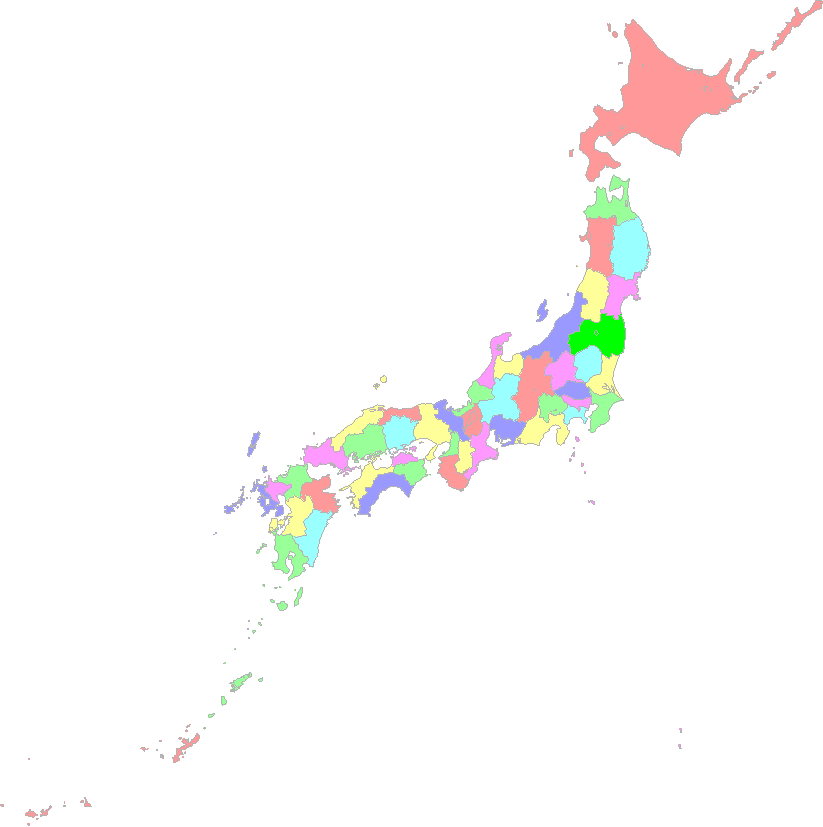
\includegraphics[scale=.4]{images/DynamicDraw01-crop}
 \caption{Dynamic Drawの描画例}\figlab{DynamicDraw}
\end{wrapfigure}

仕様書,設計書,UMLなどの作成に優れています.Dynamic Draw 単体では
\LaTeX で扱える画像形式にはならないため\footnote{今はPDFに書き出す等の
方法もあるものと思われます.},EPS Output を可能にするプラグラインも
併せてインストールしてください.ウェブページ上では種々のテンプレート
が「テンプレートライブラリ」として提供されており,UMLのテンプレート等が
公開されています.

\Hito{福代}{昌之}は上記ソフトの上位版である\Prog{Dynamic Draw
Professional}も公開されています.Professional版では,編集対象となる
文書のスナップショットを保存し,編集履歴を閲覧・検索できる\Prog{History
Manager}が含まれています.基本的にはこちらも仕様書を作成する事に特化した
ものになっているようです.


\section{Unix/Linux用の描画ソフト}

\begin{append}
 この辺に Unix系OS用の描画ソフトの解説をする.
\end{append}

\subsection{GIMP}

\begin{append}
 ここにGIMPの解説を追加する.
\end{append}


\subsection{xfig}

\begin{append}
 ここにxfigの解説を追加する.
\end{append}


\subsection{Tgif}

\begin{append}
 ここにTgifの解説を追加する.
\end{append}


\section{環境に依存しない描画ソフト}



\section{\texorpdfstring\MP MetaPost}

\ConTeXt に含まれる \TeX Exec を使うことにより \MP ファイル
\Va{file}{mp} を PDF ファイル \Va{file}{pdf} に変換するためのスクリプト。
ファイル名はイメージ順に自動的に \va{hoge}\str{-1.pdf} 等のように変換される。
\begin{InTerm}
 \type{mptopdf input.mp}
\end{InTerm}
とすれば
\begin{InText}
 beginfig (num)
 ほげほげ
 endfig;
\end{InText}
の数だけ PDF ファイルが生成されることになる。 \BB の処理もある程
度満足に良く結果となる。


\subsection{Dia}

\begin{append}
 ここにDiaの解説を追加する.
\end{append}


\subsection{OpenOffice.org Draw}

\begin{append}
 ここにOpenOffice.org Drawの解説を追加する.
\end{append}


\section{Macintosh用の描画ソフト}



\subsection{OmniGraffle}

\Prog{OmniGraffle}は\Z{The Omni Group}により販売されている描画
ソフトです.

%\begin{wrapfigure}[11]{r}{23zw}
% \centering
% 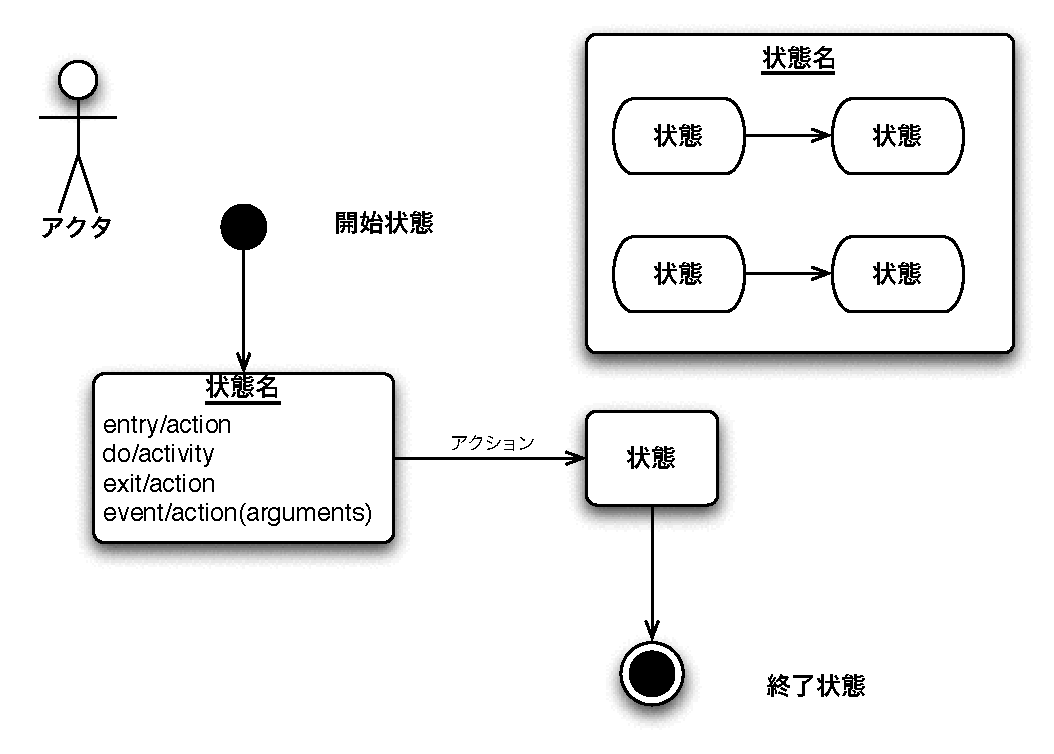
\includegraphics[scale=.4]{images/OmniGraffle00}
% \caption{OmniGraffleで作成した図の例}\figlab{omni-2}
%\end{wrapfigure}

The Omni Groupからは他にも \Prog{OmniOutliner}等が
発売されています.ユニットの連結が非常にうまくできるため,グラフやフロー
や組織図などの描画を得意とします.

ステンシルから部品となるユニットをドラッグ・ドロップする事で簡単に
色々な種類の図を作成する事が出来ます.

OmniGraffle は Standard 版と Professional 版の 2 種類があり,
Professional版ではマルチページ,マルチキャンバスやその他の機能が
搭載されています.

PDF, PNG, EPS, BMP, TIFF 等の書き出しをサポートしており,\LaTeX やプレゼ
ンツールとの連携も簡単にできるようになっています.

\image[scale=.3]{OmniGraffle01}{OmniGraffleの作業例}{omni-1}

OmniGraffleの便利な機能の一つとしてグリッドによるガイドレイアウト
があります.これは他の近隣ユニットとの整列を容易にするために,
ユニットをドラッグ中にグリッド(他のユニットとの間隔)を表示
してくれるものです\footnote{私はグリッド崇拝者なので,この機能は非常に
有り難いと思っております.早く他のソフトウェアでもグリッド指向にて
OmniGraffle並に使いやすいものを提供してほしいと切望いたします.}.

\begin{figure}[htbp]
 \centering
 \mbox{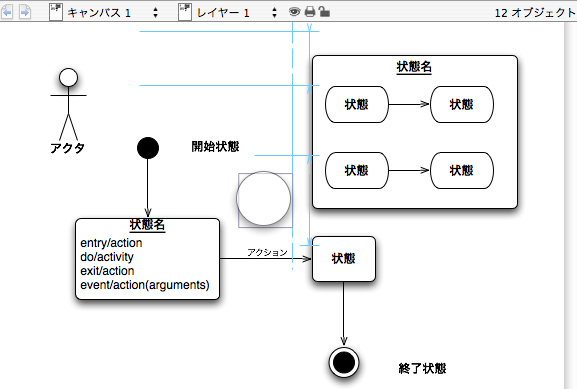
\includegraphics[scale=.4]{images/omni-grid1}~
 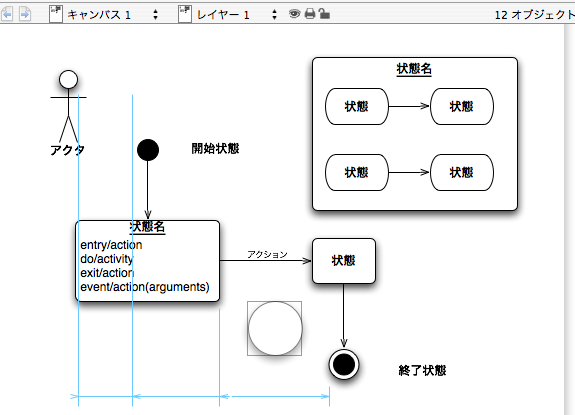
\includegraphics[scale=.4]{images/omni-grid2}}
\caption{OmniGraffleでのグリッドレイアウト}\figlab{omni-3}
\end{figure}

このガイド機能を使えば,比較的誰でも簡単に,しかも格好良くレイアウトをす
る事が出来るようになると思います.





